\chapter{TeX文書の編集}

\section{通常のコマンド}

標準的なコマンド(切り取り、コピー、検索…)は
「編集」メニューと「編集」ツールバーを通して実行できる。

\begin{figure}[H]
  \centering
  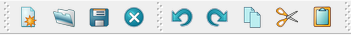
\includegraphics{doc1.png}
  \caption{標準的なコマンド}
\end{figure}

\section{TeX文書のプリアンブルの設定}

文書のプリアンブルを定義するには、(「ウィザード」メニューの)
「簡単テンプレート」ウィザードが利用できる。

\begin{figure}[H]
  \centering
  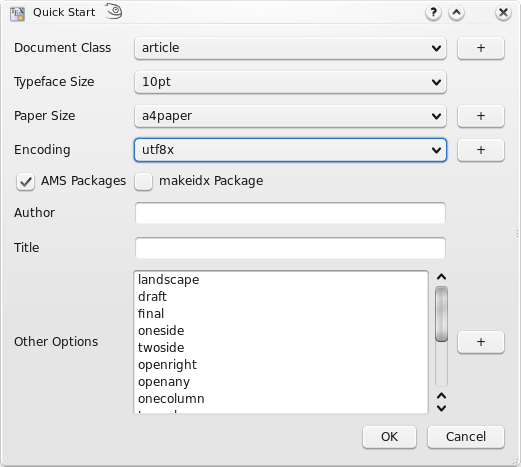
\includegraphics[width=.8\linewidth]{doc2.png}
  \caption{簡単テンプレート}
\end{figure}

このダイアログでは文書の主な仕様(文書クラス、用紙サイズ、
エンコーディング、…)を設定することができる。

注意:``+''ボタンをクリックすることで他のオプションを追加することができる。
また、設定全ては記録される。

また、エディターで自分自身のプリアンブルモデルを入力することもできる:
「コピー/貼り付け」や「名前をつけて保存」コマンドで、新規文書にそれを利用できる。

\subsection{新規文書作成時のテンプレート使用}

新規文書に対して、「ファイル/テンプレートから新規作成」コマンドを用いて
テンプレートを適応できる。
ダイアログでは利用するテンプレートを選択できる。

\begin{figure}[H]
  \centering
  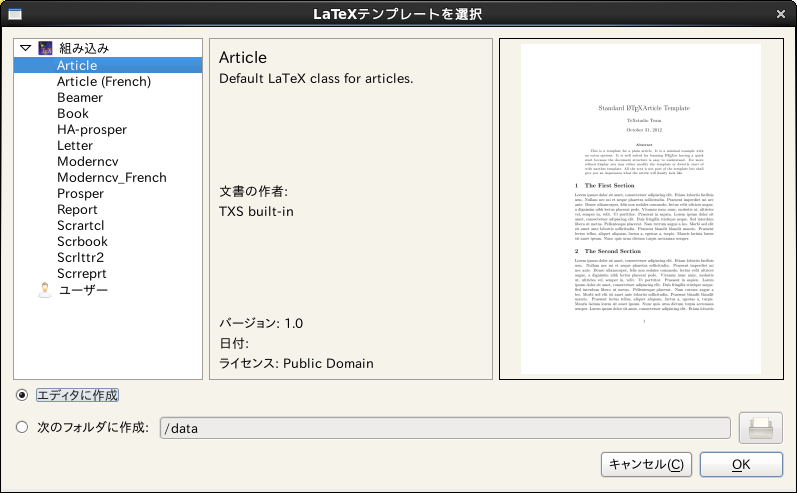
\includegraphics[width=.8\linewidth]{template.png}
  \caption{テンプレート}
\end{figure}

テンプレートから新しいエディター文書を作成するか、
テンプレートをファイルとしてディスク上に作成して
それをエディターで開くか選択することができる。
前者のオプションは複数のファイルのテンプレートに対して利用できない。

テンプレートとして利用したい開いている文書に対して、
「ファイル/テンプレートを作成」コマンドを用いて
新規テンプレートを作成することができる。
このダイアログは現在テンプレートシステムの機能すべてを
サポートしてはいないことに注意するように。
特に、プレビュー画像を提供したり、
画像つきの複数ファイルテンプレートを作成することはできない。
このようなことは手動で行う必要がある(
%\hyperref[SECTION12aa]{テンプレートの書式}
\nameref{sec:templateformat}参照)。

ユーザーが追加したテンプレートは、
テンプレート選択ダイアログでコンテキストメニューから編集や削除が可能である。
しかし、組み込みのテンプレートは変更できない。

ユーザーテンプレートは、
設定ディレクトリの\textbf{\texttt{/templates/user/}}サブディレクトリに保存される。

\subsubsection{テンプレートの書式}\label{sec:templateformat}

最も単純な形式では、テンプレートは\texttt{.tex}ファイルのみである。
複数ファイルテンプレートはすべてのファイルをzipアーカイブにまとめることで
作成することができる。
追加で、同名だが拡張子が``.tex''や``.zip''の代わりに``.json''である
別ファイルにメタデータがJSON形式で保存される。
現在次の項目がサポートされている:

\begin{lstlisting}[frame=single,breaklines=true,numbers=left]
{
"Name"        : "Book",
"Author"      : "TXS built-in",
"Date"        : "04.01.2013",
"Version"     : "1.1",
"Description" : "Default LaTeX class for books using separate files for each chapter.",
"License"     : "Public Domain",
"FilesToOpen" : "./TeX_files/chapter01.tex;main.tex"
}
\end{lstlisting}

FilesToOpenは複数ファイルの文書に対してのみ影響がある。
テンプレートファイルの隣にプレビュー画像を付け加えてもよい。
ただ、ファイル名は同名で拡張子が``.png''でなければいけない。

\section{文書構造}

TeXstudioで文書に新しい部分(節、小節、……)を定義するには、
ツールバーのこのコンボボックスを使用すれば良い:

\begin{figure}[H]
  \centering
  
\includegraphics{doc3.png}
  \caption{区分化}
\end{figure}

% これによって、その部分(節、小節、……)の体裁を定義することができる
% ダイアログがポップアップしてくる。

注:「構造ビュー」は自動的に更新される。

% \begin{figure}[H]
%   \centering
%   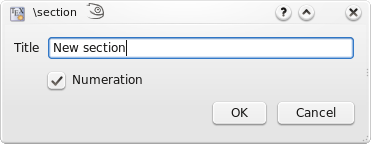
\includegraphics{doc4.png}
%   \caption{構造名入力ダイアログ}
% \end{figure}

\section{文書の閲覧}

「構造ビュー」(左側パネル)を用いると、文書のあらゆる部分にすぐに移動できる。
何らかの項目(ラベル、節、……)をクリックしさえすれば、
エディタの対応する場所の先頭へ移動する。
ある行へ移動する仕組みでは、
もはや行数を考慮するだけでなく実際のテキスト行をも記憶している。
従って、行を追加や削除しても間違った位置へ移動することはない。

灰色の背景はテキストと構造ビューでの現在のカーソル位置を示している。
緑の背景は付録での節を表している。

\begin{figure}[H]
  \centering
  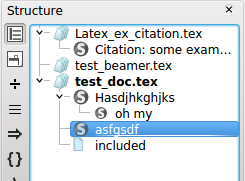
\includegraphics{doc5.png}
  \caption{構造ビュー}
\end{figure}

「構造ビュー」はタイプしたとおりに自動的に更新される。
また、いつでも(「Idefix」メニューの)「文書構造の更新」コマンドを
用いることができる。

ラベル、節、\texttt{include}や\texttt{beamer}ブロックの他に、
\verb+%TODO+で始まるコメントもスキャンされて構造ビューに項目として表示される。
これはテキストに一種の永久ブックマークを作成したり、
変更が依然として必要な場所を書き留めるために使用することができる。

また構造ビューでは、
(小節を含む)節に属するテキストすべてをコピー/切り取りして
別の節の前または後ろに貼り付けるコンテキストメニューが利用できる。
更に節のインデント/インデントの解除をすることが可能である。
それは階層構造のレベルを変更することを意味している。
つまり\verb+\section+が\verb+\subsection+に変更され、
全ての小節がそれに応じて扱われる事になる。

それぞれのファイルに対して、移動の高速化のため3つのブックマークが利用できる:
ブックマークに追加または削除するには行番号をクリックすれば良い。
すでに3つのブックマークが定義されている場合、
新たなブックマークを追加するためそのうち1つを削除しなければならない。
エディタ上でブックマークに対応する行へ移動するには、
ステータスバーのブックマークボタンをクリックすれば良い。

\begin{figure}[H]
  \centering
  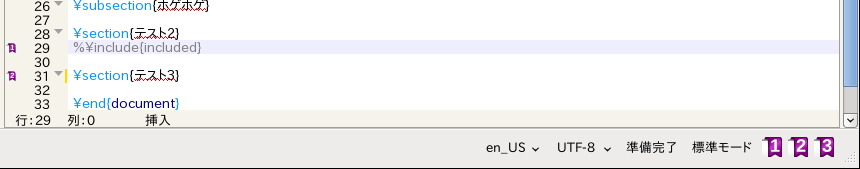
\includegraphics[width=.8\linewidth]{doc20.png}
  \caption{ブックマーク}
\end{figure}

\section{テキストの整形}

このツールバーでテキストの一部の書式を簡単に設定することができる:

\begin{figure}[H]
  \centering
  
\includegraphics{doc6.png}
  \caption{書式ツールバー}
\end{figure}

\textbf{追加のオプション:}
選択したテキストを特定の環境で直接囲うこともできる。
例:``Hello''という単語を選択した後「ボールド体」のボタンをクリックすることで、
次のコードが入力される:\verb+\textbf{Hello}+。

このオプションは「LaTeX」メニューの``{[}選択{]}''で示されている
環境全てに対して利用できる。

\subsection{大文字使用}

メニュー「編集」 -\textgreater{} 「テキスト操作」には
選択したテキストの大文字使用を変更する方法がいくつか含まれている:

\begin{itemize}
\item
  小文字化
\item
  大文字化
\item
  厳密なタイトルケース(先頭は大文字で他は小文字)化
\item
  スマートなタイトルケース(先頭は大文字で他は小文字)化
\end{itemize}

「タイトルケース化」の両方共、短い単語(a, the, ofなど)は小文字のままにする。
加えて、「スマートなタイトルケース化」は、
大文字を含む単語を大文字使用の固定を必要とする頭字語(例:「TeXstudio」)と仮定して変換しない。

\section{スペース}

通常の「スペース」コマンドは「LaTeX」と「数式」メニューで利用できる。
「強制改行」のLaTeXコマンドを簡単に挿入するには、
ツールバーの対応するコマンドを利用できる(ショートカットキー:Ctrl+return)。

\section{リストの挿入}

通常の箇条書き環境コードは「LaTeX-\textgreater{}箇条書き」メニューから
簡単に挿入できる。

注:\verb+\item+コマンドのショートカットキーはCtrl+Shift+I。

\section{表の挿入}

「表作成」ウィザード(「ウィザード」メニュー)で、
表環境に対応するLaTeXコードを簡単に挿入することができる:

\begin{figure}[htbp]
  \centering
  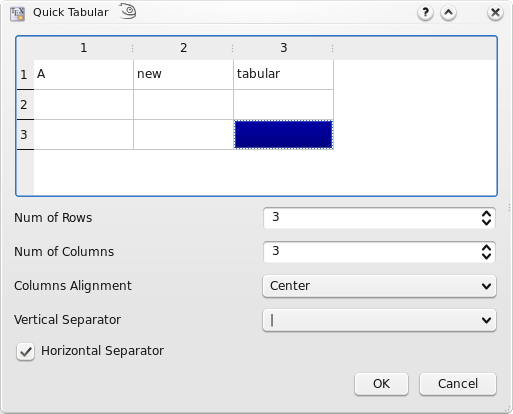
\includegraphics{doc7.png}
  \caption{表ウィザード}
\end{figure}

このウィザードで表の主な特徴を設定することができる。

注:このダイアログでセルにコードを直接入力することができる。

対応するLaTeXコードが自動的にエディタに挿入される。

\subsection{表の操作}

TeXstudioでは表を簡単に操作できるコマンドが提供されている。
そのコマンドはLaTeX → 表の操作と表ツールバーにある。
表構築のコマンドが複雑になりすぎると
予期しない結果となるかもしれないことを認識しておくこと。
次のコマンドが提供されている:

\begin{itemize}
\item
  現在の行の後ろに行を追加
\item
  行を削除:カーソルがある行を削除する
\item
  列の追加:現在のカーソル位置の後ろに列を追加する。
  カーソルが行頭(第一列)にある場合、列は新しい第一列として追加される。
\item
  列の削除:現在の列を削除する
\item
  \verb+\hline+の追加/削除:現在の行以降の全ての行に対して\verb+\hline+を追加/削除する。
  すでに\verb+\hline+のコマンドが存在している場合、
  二番目のコマンドが置かれることはない。
\item
  列の整列:列区切り記号(\&)を空白記号を挿入することで揃える。
  セルのテキストは表のヘッダーの指定に従って揃えられる。
  これは表のソースを読むのに役立つ。
\item
  テンプレートを用いて表を再構築する。
  これによって文書で同一の表の構築を行うことができる。
  いくつかのテンプレートが予め定義されており、
  java scriptのプログラミングを通して更にテンプレートを追加することができる。
  このコマンドはメニューにしか存在しない。
\end{itemize}

TeXstudioではブロックカーソルも利用できる。
\textless{}Ctrl\textgreater{}+\textless{}Alt\textgreater{}+\textless{}Shift\textgreater{}を押して
マウスでカーソルをドラッグすることで利用できる。
ブロックカーソルは通常のカーソルの組のように機能する。
通常と同じくテキストのコピーや貼り付けができる。
また新たなテキストを入力すると、全ての行にそのテキストが追加される。

\begin{figure}[H]
  \centering
  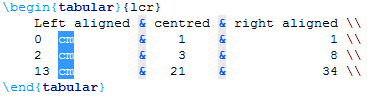
\includegraphics{block_selection.png}
  \caption{ブロック選択}
\end{figure}

\section{``tabbing''環境の挿入}

``tabbing''コードを挿入するのを容易に行うため、
(「ウィザード」メニューの)``Tabbing''ウィザードを利用できる:

\begin{figure}[H]
  \centering
  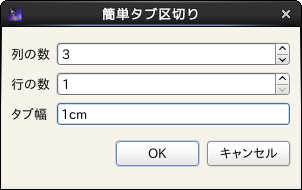
\includegraphics{doc8.png}
  \caption{Tabbingウィザード}
\end{figure}

\section{図の挿入}

文書中に図を挿入するには、
「LaTeX」メニューの``\verb+\includegraphics+''コマンドを使用すれば良い。
そして画像ファイルを選択するためダイアログの「ブラウザ」ボタンをクリックすれば良い。

注:図の挿入前に(「LaTeX - 環境」メニューの)``figure'' LaTeX環境を挿入してもよい。

\begin{figure}[H]
  \centering
  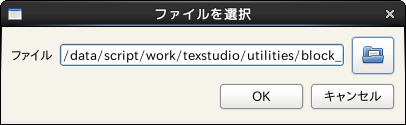
\includegraphics{doc9.png}
  \caption{図環境}
\end{figure}

\subsection{「ウィザード」を用いた図の挿入}

図の適切な挿入は、LaTeX初心者には挑戦であり、
熟練者にはほんの僅かのテキストをタイプすることである。
従ってTeXstudioでは文書への画像挿入コードを扱うウィザードを提供している。
「画像オプション」では
\textbf{\texttt{\textbackslash{}includegraphics[options]\{file\}}}の
オプションパラメータを定義する。
最も使用される幅/高さの属性は容易に設定できる一方で、
ユーザー定義の設定で完全に制御することもできる。

画像をテキスト中のまさにその位置に配置する必要がない場合、
画像を\textbf{\texttt{figure}}環境内に置くべきだ。
そしたらLaTeXの方でページ上の最適な位置を決定してくれる。

「既定として保存」ボタンを押すことで、
現在の設定(ファイル、図見出し、ラベルを除く)が保存される。
そしてウィザードを開いた際その設定を既定として使用することができるようになる。

画像ファイルを文書にドラッグ&ドロップしたり、
エクスプローラーでコピーしてTeXstudioで貼り付けたりした時にも、
画像挿入ウィザードが起動する。
これによって、調整可能な既定パラメータを伴って新しい画像を非常に素早く挿入できる。
更に図のコード上にカーソルがあるときに画像挿入ウィザードを開始すると、
既存の図の設定をそのウィザードで操作することができる。

\begin{figure}[H]
  \centering
  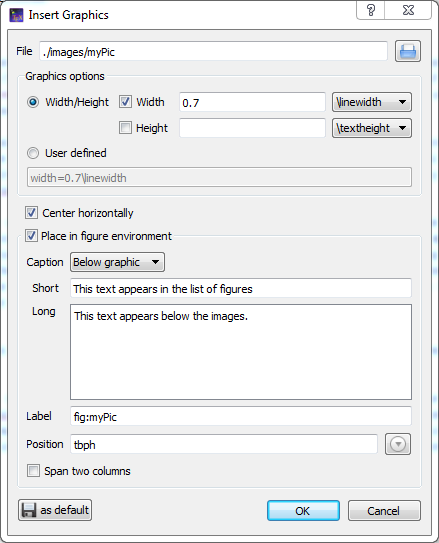
\includegraphics{wizard_figure.png}
  \caption{図ウィザード}
\end{figure}

\section{相互参照及び注釈}

ツールバーのこのツールボックスでラベルや引用、参照、脚注などの
コードをすぐに挿入できる。

注:文書中で用いられているラベルは「構造ビュー」に表示される。

\begin{figure}[H]
  \centering
  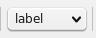
\includegraphics{doc10.png}
  \caption{ラベルなどのツールボックス}
\end{figure}

\textbf{追加のオプション:}\verb+\ref+コマンドに対しては、
ダイアログボックスで直接ラベルを選択することができる。

\section{数式の挿入}

ツールバーの「インライン数式」ボタン(ショートカット:Ctrl+Shift+M)または
「数式」メニューで、「インライン数式」環境内の状態へと切り替えることができる。
「ディスプレイ数式」環境のショートカットキーは次である:Alt+Shift+M。

「数式」ツールバーで\verb+\left+や\verb+\right+タグのような
最も使用される数学的な形(frac, sqrt\ldots{})を挿入できる。

\begin{figure}[H]
  \centering
  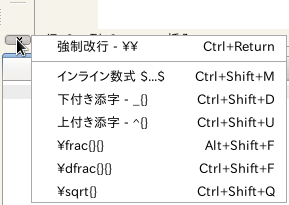
\includegraphics{doc11.png}
  \caption{数式ツールバー}
\end{figure}

また、「文書の構造」ビューの「記号パネル」を用いて、
400種類の数学記号のコードを挿入することができる。

\begin{figure}[H]
  \centering
  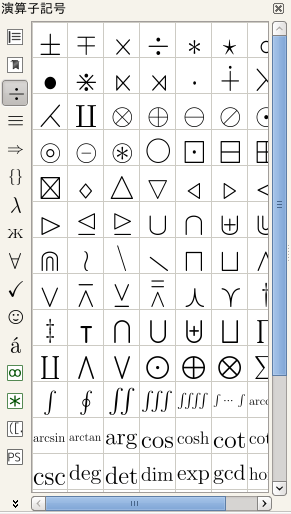
\includegraphics{doc12.png}
  \caption{数学記号パネル}
\end{figure}

「数式」メニューを通して数学的テキストの書式を決めることもできる。

``array''環境に対しては、(「表」ウィザードのように)
「ウィザード」メニューからウィザードが利用できる。
このウィザードでは、使用する環境(array, matrix, pmatrixなど)を
選択することができる。
更にセルを直接埋めることもできる。

\begin{figure}[H]
  \centering
  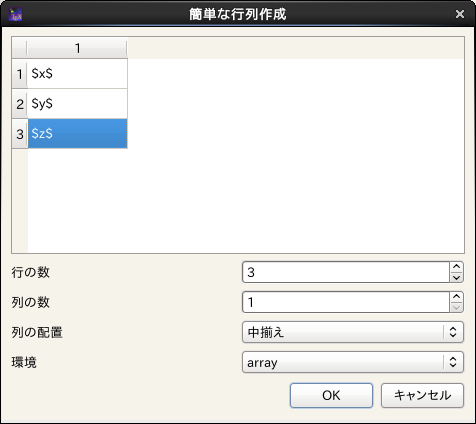
\includegraphics{doc13.png}
  \caption{行列ウィザード}
\end{figure}

\section{自動補完}

``\textbackslash{}''に続いて文字を打つと常に、
考えられるLaTeXタグのリストが表示され、正しいものを選択することができる。
追加の文字を打った場合、LaTeXタグリストはフィルター処理されて、
すでに書かれたテキストで始まるタグのみが表示される。
タグリストが同じ文字の組み合わせで始まる単語だけを含む場合、
Tabキーを押して全てに共通する文字を補完することができる。
もしタグリストに一つしか要素がない場合、
EnterキーのようにTabキーでこれを選択して補完することができる。
この振る舞いはbashシェルでのtab補完に似ている。
また、望むときにCtrl+Spaceを押してこのタグリストを開くことも可能である。

タグに異なるオプションがある場合、短い説明的なテキストが挿入され、
それぞれのオプションの意味を教える。
更に、Ctrl+LeftとCtrl+Rightを押してあらゆる位置を選択することができる。

また通常のテキストも単語をタイプし始めてCtrl+Spaceを押すことで
補完を行うことができる。
現在の文書の適切な単語全てが考えられる候補として用いられる。

環境を挿入するつもりであれば、環境名の最初をタイプしてCtrl+Alt+Spaceを押すことで、
適切な環境の候補が表示されて\verb+\begin{env}+..\verb+\end{env}+で
補完挿入される。

そして最後に、ユーザータグを補完で使用することもできる
略語へ割り当てることが可能である。
略語の最初の部分をタイプしてCtrl+Spaceで補完を開始するだけでよい。
そうした略語は、特に``略語(テンプレート)''でしるし付けされて
補完リストに表示される。

もし新たなコマンドを補完することでとあるコマンドを変える場合、
コマンド名のみが取り替えられる。
同じことが環境に対しても当てはまり、\verb+\begin+- \& \verb+\end+-コマンド内の
環境名が変化する。

\section{類語辞典}

TeXstudioは単純な類語辞典を統合している。
これにはOpenOffice 2.xのデータベースを使用している。
単語上にカーソルを置いて類語辞典を
アクティブにする(Ctrl+Shift+F8またはツール/類語辞典)ことで、
この単語に対する類義語を見つけようとする。
類語辞典を初めて起動する場合には、
データベースの読み込みが生じて少し時間がかかりうるので我慢すること。

\begin{figure}[H]
  \centering
  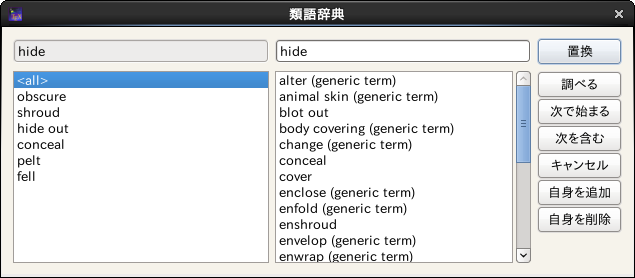
\includegraphics[width=.8\linewidth]{thesaurus.png}
  \caption{類語辞典}
\end{figure}

左側の最初の行は類義語を探索する対象単語を含む。
その下のリストは単語の種類のリストである。
それらのいずれかを選択して候補の数を減らすことができる。
右側の欄は提案された類義語のリストを含む。
このリストから選択した単語が、
そのテキストの代わりに対する提案として右側の最初の行に表示される。
この単語は手動で変更できる。
その単語は、それ「で始まる」またはそれ「を含む」単語や類義語に対する
さらなる調査にも用いられる。
「調べる」でその単語の類義語を探すために直接利用することもできる。

\section{特殊コマンド}

\subsection{単語/コマンド/環境の削除}

Alt+Delのショートカットでカーソル位置の単語が削除される。
それがコマンドならば、そのコマンドが開き括弧と閉括弧を含んで削除される。
例:``\verb+\textbf{text}+''は``text''が残ることになる。
もしも環境だった場合、取り囲むbegin/endが削除される。

\subsection{環境名の付け替え}

カーソルが環境名もしくは対応するbegin-/end-コマンド上にある場合、
少ししてミラーカーソルがアクティブになる。
これでbegin-\&end-コマンドの環境名を同時に変更することができる。
もし``\verb+\begin{tabular}+\ldots{}\verb+\end{tabular}+''構文
を``\verb+\begin{tabularx}+\ldots{}\verb+\end{tabularx}+''へ変更したい場合、
テキストカーソルを``tabular''の上に置き
「環境名の付け替え」を実行して少し待てばよい。
すると、ミラーカーソルが現れて``tabular''を``tabularx''に変更できるようになる。

\subsection{バッファの切り取り}

何かを選択してコマンドを入力し始めて補完を行う場合、
選択したものが最初の引数として配置される。
例:``text''があり、それを選択して``\verb+\textbf+''を補完入力する。
すると結果として得られるテキストは``\verb+\textbf{text}+''となる。
